\documentclass[journal]{IEEEtran}
\usepackage{graphicx}
\usepackage{caption}
\usepackage{cite}


	\begin{document}
		
		\title{Depth Estimation\\ {\Large using Stereo Camera Calibration}}
		\author{Croco Marine,~\IEEEmembership{Team,~ROV}}
	
	
	
	% The paper headers
	\markboth{Journal of CrocoMarine\,~Vol.~1, No.~1, ec~2023}%
	{Shell \MakeLowercase{\textit{et al.}}: Bare Demo of IEEEtran.cls for IEEE Journals}
	\maketitle
	
	% As a general rule, do not put math, special symbols or citations
	% in the abstract or keywords.
	\begin{abstract}
		Measuring the lenght of unknown objects has always been a feature we seek to achive, in this article we will dicuss how we will do measurement using only two adjacent cameras.  
	\end{abstract}
	
	\begin{IEEEkeywords}
		Stereo Camera, Depth maps.
	\end{IEEEkeywords}
	
	
	\IEEEpeerreviewmaketitle
	
	
	\section{Introduction}
	\IEEEPARstart{I}{n} the preliminary phase of our research focused on underwater environmental measurement, we initially contemplated utilising reference points to aid our data collection efforts. However, the scarcity of viable reference points submerged in aquatic environments presented a formidable obstacle to our objectives. Following a thorough investigative and exploratory process, we identified a pragmatic solution: the incorporation of depth cameras for data acquisition.
	
	Regrettably, the accessibility of commercially available depth cameras within our region was limited, and the associated costs were exorbitant. In response to this logistical challenge, we resolved to embark on a comprehensive endeavour aimed at developing our own custom depth camera system. This strategic decision allowed us to address the scarcity of suitable equipment and positioned us to meet the specific demands of our underwater measurement applications.
	
	\section{Process}
	\subsection{Camera alignment and Calibration}
	In the initial phase of our project, we endeavoured to achieve precise horizontal alignment between two cameras. However, our efforts were hindered by inherent mechanical constraints, preventing us from attaining absolute {100\%} alignment accuracy. As part of our investigative process, we encountered and subsequently adopted stereo calibration and rectification methodologies. These techniques have empowered us to leverage triangulation principles, thereby facilitating the precise calculation of 3D coordinates for objects displayed on the screen. This technological approach enhances the accuracy and reliability of our system for capturing and analysing 3D spatial information.
	
	Our validation process for the depth camera involved the generation of a depth map utilising HitNet, a neural network-based solution. The results demonstrated a high level of accuracy and proficiency in depth estimation, as exemplified in the accompanying image.\\
	
	Figure \ref{fig:stereo output} shows stereo camera calibration output.
	\begin{figure}[h]
	\centering
		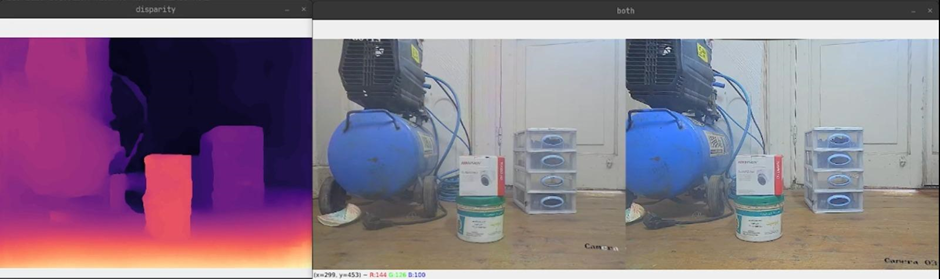
\includegraphics[width=\linewidth]{stereo camera output vs generated depth heat map.png}
		\caption{stereo camera output vs generated depth heat map}
		\label{fig:stereo output}
	\end{figure}
	
	
	\subsection{3D Measurment Algorithm}
		Rather than solely relying on the depth map for XYZ point calculations, we opted for a more intricate triangulation algorithm.\\
		This algorithm necessitates the input of four distinct points and, in turn, provides an output representing the spatial distance between lines in the 3D world. This approach offers enhanced precision in our measurements and is crucial for our specific applications.\\
		
		Figure \ref{fig:triangulation from the projections of P onto two images.} shows the 3D location of a point P can be computed by triangulation from the projections of P onto two images.
		
		\begin{figure}[h]
			\centering
			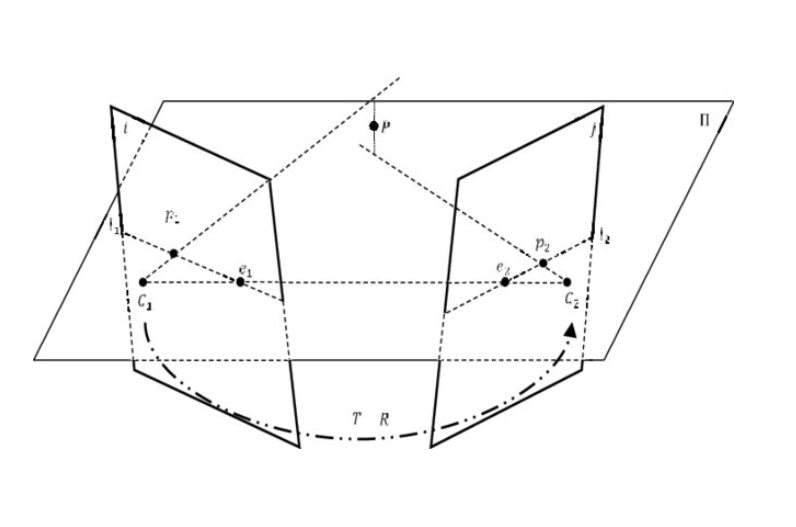
\includegraphics[width=\linewidth]{ triangulation from the projections of P onto two images.png}
			\caption{triangulation from the projections of P onto two images.}
			\label{fig:triangulation from the projections of P onto two images.}
			\cite{inproceedings}
		\end{figure}

	\section{Results}
	
	 The testing of this triangulation algorithm involved applying it to a stereo photograph of a fish taken by our camera system.
	 
	 The algorithm yielded a measurement of 22.17 centimetres, while the actual physical measurement stood at 22 centimetres, resulting in an impressively minimal margin of error, less than 2 millimetres. This level of accuracy underscores the effectiveness of our approach in providing highly precise 3D measurements.\\
	 
 	Figure \ref{fig:the actual length of the object in printed image vs the estimated} shows the estimated length of the fish presented in the printed image(in red) vs the actual written along the image(in blue).
	 \begin{figure}[h]
	 	\centering
	 	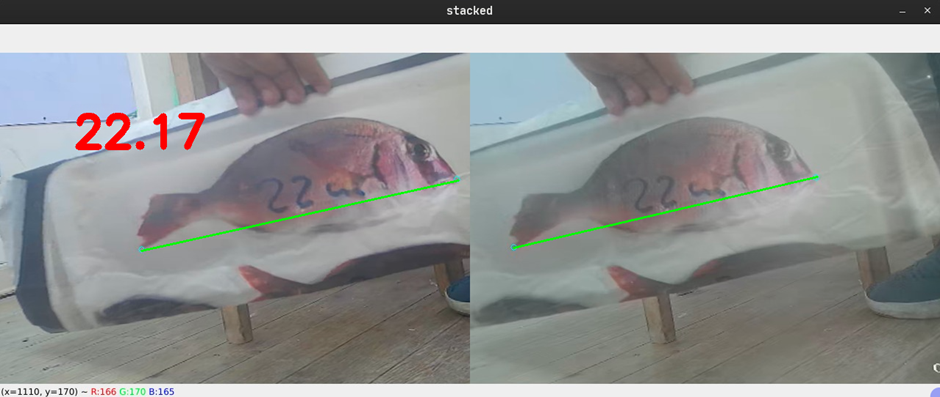
\includegraphics[width=\linewidth]{Output of the algorithm.png}
	 	\caption{the output of triangilation algorithm on known lenght fish printed image.}
	 	\label{fig:the actual length of the object in printed image vs the estimated}
	 \end{figure}
	 

	\section{Conclusion}
	 With the use of two stereo calibrated cameras we could precisely estimate length of the seen objects.  

	
	\ifCLASSOPTIONcaptionsoff
	\newpage
	\fi
		
	\bibliographystyle{IEEEtran}
	\bibliography{citation}
\end{document}


